\begin{enumerate}
	\item D'après l'énoncé, si elle vient de gagner une partie, elle gagne la suivante dans 70\% des cas, elle perd donc la suivante dans 30\,\%.

On a donc $P_{G_1}(D_2)=0,3$


	\item


	On a l'arbre suivant :

	\begin{center}
		\hfill~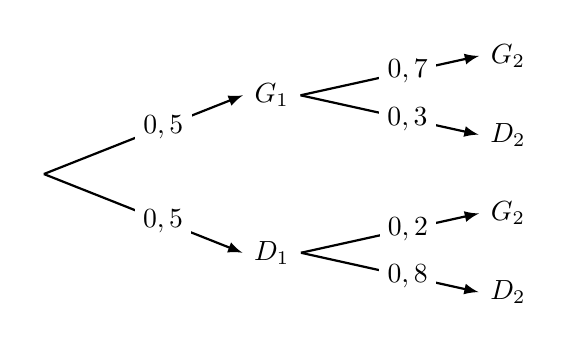
\begin{tikzpicture}[xscale=1,yscale=1,baseline={(R.base)}]
			
			\tikzstyle{fleche}=[->,>=latex,thick]
			\tikzstyle{noeud}=[fill=white,circle,inner sep=2pt]
			\tikzstyle{feuille}=[fill=white,circle,inner sep=2pt]
			\tikzstyle{etiquette}=[pos=0.6,fill=white, inner xsep=3pt, inner ysep=1.5pt]
			
			\def\DistanceInterNiveaux{3}
			\def\DistanceInterFeuilles{1}
			
			\def\NiveauA{(0)*\DistanceInterNiveaux}
			\def\NiveauB{(1)*\DistanceInterNiveaux}
			\def\NiveauC{(2)*\DistanceInterNiveaux}
			\def\InterFeuilles{(-1)*\DistanceInterFeuilles}
			
			\node[noeud] (R) at ({\NiveauA},{(1.5)*\InterFeuilles}) {};
			\node[noeud] (Ra) at ({\NiveauB},{(0.5)*\InterFeuilles})            {$G_1$};
			\node[feuille] (Raa) at ({\NiveauC},{(0)*\InterFeuilles})           {$G_2$};
			\node[feuille] (Rab) at ({\NiveauC},{(1)*\InterFeuilles}) {$D_2$};
			\node[noeud] (Rb) at ({\NiveauB},{(2.5)*\InterFeuilles})  {$D_1$};
			\node[feuille] (Rba) at ({\NiveauC},{(2)*\InterFeuilles})           {$G_2$};
			\node[feuille] (Rbb) at ({\NiveauC},{(3)*\InterFeuilles}) {$D_2$};
			
			\draw[fleche] (R.east)--(Ra.west) node[etiquette]   {$0,5$};
			\draw[fleche] (Ra.east)--(Raa.west) node[etiquette] {$0,7$};
			\draw[fleche] (Ra.east)--(Rab.west) node[etiquette] {$0,3$};
			\draw[fleche] (R.east)--(Rb.west) node[etiquette]   {$0,5$};
			\draw[fleche] (Rb.east)--(Rba.west) node[etiquette] {$0,2$};
			\draw[fleche] (Rb.east)--(Rbb.west) node[etiquette] {$0,8$};
		\end{tikzpicture} \hfill~	\end{center}


	\item   Les évènements $G_1$ et $D_1$ partitionnent l'univers, donc, d'après la loi des probabilités totales, on a :

	$\begin{aligned} g_2=P(G_2) &= P(G_1 \cap G_2) + P(D_1 \cap G_2)\\
	&= 0,5\times 0,7 +0,5\times 0,2 \\
	&= 0,35+0,1\\
	&= 0,45\end{aligned}$

	\item
	\begin{enumerate}
		\item On a l'arbre suivant :

		\begin{center}
		\hfill~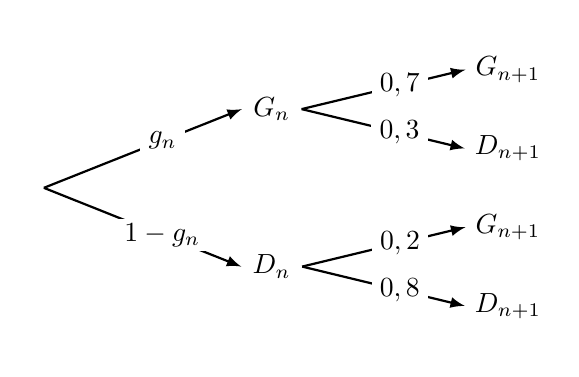
\begin{tikzpicture}[xscale=1,yscale=1,baseline={(R.base)}]
		
		\tikzstyle{fleche}=[->,>=latex,thick]
		\tikzstyle{noeud}=[fill=white,circle,inner sep=2pt]
		\tikzstyle{feuille}=[fill=white,circle,inner sep=2pt]
		\tikzstyle{etiquette}=[pos=0.6,fill=white, inner xsep=3pt, inner ysep=1.5pt]
		
		\def\DistanceInterNiveaux{3}
		\def\DistanceInterFeuilles{1}
		
		\def\NiveauA{(0)*\DistanceInterNiveaux}
		\def\NiveauB{(1)*\DistanceInterNiveaux}
		\def\NiveauC{(2)*\DistanceInterNiveaux}
		\def\InterFeuilles{(-1)*\DistanceInterFeuilles}
		
		\node[noeud] (R) at ({\NiveauA},{(1.5)*\InterFeuilles}) {};
		\node[noeud] (Ra) at ({\NiveauB},{(0.5)*\InterFeuilles})            {$G_n$};
		\node[feuille] (Raa) at ({\NiveauC},{(0)*\InterFeuilles})           {$G_{n+1}$};
		\node[feuille] (Rab) at ({\NiveauC},{(1)*\InterFeuilles}) {$D_{n+1}$};
		\node[noeud] (Rb) at ({\NiveauB},{(2.5)*\InterFeuilles})  {$D_n$};
		\node[feuille] (Rba) at ({\NiveauC},{(2)*\InterFeuilles})           {$G_{n+1}$};
				\node[feuille] (Rbb) at ({\NiveauC},{(3)*\InterFeuilles}) {$D_{n+1}$};
				
		\draw[fleche] (R.east)--(Ra.west) node[etiquette]   {$g_n$};
		\draw[fleche] (Ra.east)--(Raa.west) node[etiquette] {$0,7$};
		\draw[fleche] (Ra.east)--(Rab.west) node[etiquette] {$0,3$};
		\draw[fleche] (R.east)--(Rb.west) node[etiquette]   {$1-g_n$};
		\draw[fleche] (Rb.east)--(Rba.west) node[etiquette] {$0,2$};
		\draw[fleche] (Rb.east)--(Rbb.west) node[etiquette] {$0,8$};
		\end{tikzpicture} \hfill~	\end{center}

		\item  Pour tout entier naturel $n$ non nul, les évènements $G_n$ et $D_n$ déterminent  une partition de l'univers, donc, d'après la loi des probabilités totales, on a :

$\begin{aligned} g_{n+1}=P(G_{n+1}) &= P(G_n\cap G_{n+1}) + P(D_n \cap G_{n+1})\\
&= g_n\times 0,7 +(1-g_n)\times 0,2 \\
&= 0,7g_n+0,2- 0,2g_n\\
&= 0,5g_n+0,2\end{aligned}$

On arrive bien au résultat annoncé.

	\end{enumerate}
	\item
	\begin{enumerate}
		\item  Soit $n$ un entier non nul.

		$\begin{aligned} v_{n+1}& = g_{n+1}-0,4 \quad \text{par définition de la suite } \left(v_n\right)\\
		&= 0,5g_n+0,2-0,4 \quad \text{par définition de la suite } \left(g_n\right)\\
		&= 0,5 ( v_n+0,4) -0,2 \quad \text{car } v_n=g_n-0,4 \iff g_n=v_n+0,4\\
		&= 0,5 v_n +0,2-0,2\\
		&=0,5v_n\end{aligned}$

		La suite $ \left(v_n\right)$ est donc une suite géométrique de raison $q = 0,5$ et de premier terme \linebreak$v_1 = g_1 - 0,4 = 0,5 - 0,4 = 0,1$


		\item  On peut donc en déduire que pour tout entier naturel $n$ non nul :

		$v_n=v_1\times q^{n-1}= 0,1 \times 0,5^{n-1}$

		Or pour tout entier naturel n non nul \quad $g_n=v_n+0,4$ \quad donc \quad $g_n=0,1 \times 0,5^{n-1}+0,4$.

	\end{enumerate}
	\item   Soit $n$ un entier naturel non nul.

	$\begin{aligned} g_{n+1}-g_{n}&=0,1 \times 0,5^{n}+0,4-0,1 \times 0,5^{n-1}-0,4\\
	&= 0,1 \times 0,5^{n-1} \times ( 0,5-1)\\
	&= 0,1 \times 0,5^{n-1} \times (-0,5)\\
	&= -0,1 \times 0,5^n\end{aligned}$

	or $0,5 > 0$ et $0,1> 0$ donc $g_{n+1}- g_{n}< 0 \iff g_{n+1} <  g_{n}$

	La suite $\left(g_n\right)$ est strictement décroissante.


	\item   $-1 < 0,5<1$, donc on en déduit $\lim\limits_{n \to +\infty} \left(0,5\right)^n = 0$, donc, par limite du produit et de la somme : $\lim\limits_{n \to +\infty} 0,1 \times 0,5^{n-1}+0,4 = 0,4$.

	Sur le long terme, Léa gagnera son match dans 40\,\% des cas.
	\item  Déterminons les valeurs de $n$ pour lesquels  $g_n-0,4\leqslant 0,001$

	$\begin{aligned} g_n-0,4\leqslant 0,001 & \iff 0,1 \times 0,5^{n-1}+0,4 -0,4 \leqslant 0,001 \\
	&\iff 0,1 \times 0,5^{n-1} \leqslant 0,001 \\
		&\iff 0,5^{n-1} \leqslant 0,01 \quad \text {car } 0,1>0\\
	&\iff \ln\left( 0,5^{n-1} \right)\ \leqslant \ln(0,01) \quad \text{par croissance de la fonction } \ln \text{ sur }\R^{*+}\\
	&\iff(n-1) \ln\left( 0,5 \right) \leqslant \ln(0,01) \\
	&\iff(n-1) \geqslant \dfrac{\ln(0,01)}{\ln(0,5)} \quad \text {car } \ln(0,5)<0\\
	&\iff n \geqslant \dfrac{\ln(0,01)}{\ln(0,5)} +1 	\end{aligned}$


	Or  $\dfrac{\ln(0,01)}{\ln(0,5)} +1 = \dfrac{-\ln(100)}{-\ln(2)} + 1 = \dfrac{\ln(100)+ \ln(2)}{\ln(2)} = \dfrac{\ln(200)}{\ln(2)} \approx 7,64$ donc, $n$ étant un entier, la plus petite valeur de $n$ tel que $g_n-0,4\leqslant 0,001$ est 8.

	\item Le programme complété est :

	\begin{center}
		\ttfamily
		\begin{tabularx}{10cm}{|X|}\hline
			def seuil(e):\\
			\quad g = 0.5\\
			\quad n = 1\\
			\quad while {g \red > 0.4 + e} :\\
			\quad \quad g =  0.5 * g + 0.2\\
			\quad \quad n = {\red n + 1}\\
			\quad return(n)\\ \hline
		\end{tabularx}
	\end{center}
\end{enumerate}
